\documentclass[11pt]{article}
\usepackage[margin=1in]{geometry}
\usepackage{amsmath,amssymb,bm}
\usepackage{booktabs,multirow}
\usepackage{graphicx}
\usepackage{hyperref}
\hypersetup{pdftitle={How Should Measurements Enter Flow-Matching ODE Sampling? A Controlled Study for Sparse-View and Low-Dose CT}}
\usepackage{xcolor}
\usepackage{placeins}
\usepackage[numbers,sort&compress]{natbib}

\newcommand{\A}{\mathcal{A}}
\newcommand{\x}{\bm{x}}
\newcommand{\y}{\bm{y}}
\newcommand{\vel}{\bm{v}_\theta}

\title{How Should Measurements Enter Flow-Matching ODE Sampling?\\
A Controlled Study for Sparse-View and Low-Dose CT}
\author{Weihao Zhang\\
  Hebei University, Baoding, China\\
  \texttt{20268018055@stumail.hbu.edu.cn}}
\date{}

\begin{document}
\maketitle

\begin{abstract}
Flow-matching priors are increasingly used for CT reconstruction, but published methods differ simultaneously in the
prior, the network, the data and the rule that injects the measurements, which makes it hard to know what actually
matters. We hold everything fixed except that rule. On a single 19.8M-parameter rectified-flow prior trained on the
public TotalSegmentator CT collection (1228 volumes, official patient-level split), we compare gradient guidance
(DPS-style), pseudo-inverse guidance ($\Pi$GDM-style) and proximal data consistency (DDS/DDNM-style) inside the same
Euler ODE integrator, against FBP and a supervised FBPConvNet with the same backbone, for 30/60/90-view and low-dose
parallel-beam CT. Guidance strengths are expressed in units that are invariant to the number of steps and of views,
and are selected on validation patients only; all comparisons use patient-level bootstrap confidence intervals.
Three findings stand out. (i) Pseudo-inverse guidance gives the best single samples from 60 views (36.9\,dB, $+1.4$\,dB
over FBPConvNet, 95\% CI $[0.95,1.91]$), while proximal consistency is the most step-efficient (36.2\,dB at 20 steps) and
gives the best posterior means ($+3.9$\,dB over FBPConvNet with 8 samples). (ii) DPS-style guidance fails on the flow ODE: it saturates at $\approx 24.5$\,dB irrespective of the number of views and
hallucinates anatomy; a preliminary measurement shows its gradient varying by about $60\times$ along the trajectory.
(iii) Under photon noise, without an explicit noise model, the supervised baseline remains better (+2.2\,dB at
$I_0{=}10^5$), and with strengths transferred (not re-tuned) from $I_0{=}10^5$ the ranking inverts at $I_0{=}10^4$. Code, configurations and per-image results are available at \url{https://github.com/ZeroDevi1/flow-ct-guidance}.
\end{abstract}

\section{Introduction}
Generative priors have become a strong alternative to supervised post-processing for ill-posed CT reconstruction:
one unconditional prior can be reused across acquisition protocols, and posterior sampling exposes uncertainty that
a deterministic network hides~\cite{song2022scoremed,chung2022mcg,chung2023dps}. Most of this literature is built on
diffusion SDEs. Flow matching and rectified flow~\cite{lipman2023flow,liu2023rectified} instead learn a velocity field
whose ODE transports noise to data along nearly straight paths. This makes few-step sampling attractive, but it also
changes \emph{where} and \emph{how strongly} measurement information should be injected, because there is no per-step
stochastic re-noising to absorb guidance errors.

Flow priors for CT are now an active topic~\cite{evangelista2026pgfm,shi2026dm4ct,eFMCT2026,lucid2026}, and generic flow
solvers adapt diffusion guidance in several ways~\cite{pokle2024otode,martin2025pnpflow,kim2025flowdps}. Most of these studies change the prior, the network, the data or the step schedule together with the guidance rule;
Evangelista~\cite{evangelista2026pgfm} does compare several flow solvers on one prior (Mayo LDCT), but without step- and
view-invariant units for the guidance strength, validation-only tuning or patient-level confidence intervals. Guidance
weights are usually tuned heuristically, which recent work shows to be decisive~\cite{moroy2026guidanceweights,barthakur2026leegs}.
We therefore isolate the single factor of \emph{how measurements enter the ODE}. With one flow-matching prior trained on
TotalSegmentator CT~\cite{wasserthal2023totalseg}, we compare (M1) a DPS-style gradient step through the
network~\cite{chung2023dps}, (M2) a $\Pi$GDM-style pseudo-inverse correction~\cite{song2023pigdm} and (M3) a
conjugate-gradient proximal projection of the predicted clean image~\cite{chung2024dds}. All three share the prior, the
integrator, the number of function evaluations (NFE), the validation-based tuning protocol and the test set, and are
compared with FBP and with a supervised FBPConvNet~\cite{jin2017fbpconvnet} that uses the same backbone.

\paragraph{Contributions.}
\begin{itemize}
  \item A controlled comparison of three measurement-injection rules on a shared rectified-flow prior for sparse-view
        (30/60/90 views) and low-dose CT on public data, with validation-only tuning and patient-level bootstrap
        intervals (Tables~\ref{tab:main},~\ref{tab:mean}).
  \item Unit conventions that make guidance strengths comparable across NFE and across view counts---the DPS step is
        scaled by $\Delta t$ and by $1/\sqrt{\operatorname{tr}(\A^\top\A)/N^2}$, and the proximal weight is expressed relative
        to $\operatorname{tr}(\A^\top\A)/N^2$---which would otherwise confound NFE ablations and cross-protocol comparisons.
  \item Evidence that gradient guidance does not exploit additional views on the flow ODE (a view-independent plateau,
        with a preliminary measurement of a $\sim\!60\times$ variation of the guidance gradient along the trajectory),
        and that pseudo-inverse and proximal rules have different uncertainty behaviour, which reverses their ranking
        between single samples and posterior means.
\end{itemize}

\section{Related work}
\paragraph{Diffusion posterior sampling.}
DPS~\cite{chung2023dps} and MCG~\cite{chung2022mcg} back-propagate a measurement loss through the denoiser;
$\Pi$GDM~\cite{song2023pigdm} replaces the gradient by a pseudo-inverse correction under a Gaussian approximation of
$p(\x_0\mid\x_t)$; DiffPIR~\cite{zhu2023diffpir}, DDS~\cite{chung2024dds} and DAPS~\cite{zhang2025daps} alternate between
denoising and a proximal or data-consistency step; RED-diff~\cite{mardani2024reddiff} casts sampling as variational
optimisation. For CT specifically, score-based priors~\cite{song2022scoremed}, DiffusionMBIR~\cite{chung2023diffusionmbir},
DiffusionBlend~\cite{song2024diffusionblend} and DOLCE~\cite{liu2023dolce} address sparse-view, 3-D and limited-angle settings.
DM4CT~\cite{shi2026dm4ct} benchmarks ten diffusion methods for CT; our study is complementary: it fixes a flow prior and
varies only the injection rule.
\paragraph{Flow priors for inverse problems and CT.}
OT-ODE~\cite{pokle2024otode} derives $\Pi$GDM-like corrections for conditional OT paths, PnP-Flow~\cite{martin2025pnpflow}
interleaves flow denoising with plug-and-play projections, and FlowDPS~\cite{kim2025flowdps} decomposes the flow update into
clean-image and noise components. For CT, Evangelista~\cite{evangelista2026pgfm} trains a rectified-flow prior on Mayo LDCT
and compares several flow solvers with diffusion baselines; EFMCT~\cite{eFMCT2026} reuses velocity fields across steps
together with data consistency; LUCID~\cite{lucid2026} adapts the trajectory to the sparsity level and corrects in the
projection domain. Guidance-weight selection has recently been addressed by offline least squares~\cite{moroy2026guidanceweights}
and by learned schedules~\cite{barthakur2026leegs,bang2026trips}. We differ in scope: a single prior, three injection rules,
step- and view-invariant units, validation-only tuning on a public dataset, and patient-level statistics.
\paragraph{Supervised CT reconstruction.}
FBPConvNet~\cite{jin2017fbpconvnet} and LEARN~\cite{chen2018learn} learn a mapping from under-sampled data; they are strong
in-distribution but must be retrained per protocol.

\section{Method}
\subsection{Imaging model}
An axial slice $\x\in[-1,1]^{N\times N}$ ($N{=}256$, HU window $[-1000,1000]$) is mapped to attenuation
$u = m\odot(\x+1)/2$, where $m$ is the inscribed-disk mask. The parallel-beam projector $R_\Theta$ samples
$|\Theta|$ equispaced angles in $[0,\pi)$; the forward model is affine in $\x$,
\begin{equation}
  \A(\x) = R_\Theta(u) = \A_{\mathrm{lin}}\x + \bm{b},\qquad \A_{\mathrm{lin}}\x = R_\Theta(m\odot\x/2),\quad \bm b = R_\Theta(m/2).
\end{equation}
$R_\Theta$ is implemented by rotation with bilinear interpolation followed by summation; its exact adjoint is obtained by
automatic differentiation (relative adjoint error $<10^{-4}$, unit-tested). Sparse-view data use
$|\Theta|\in\{30,60,90\}$ (full sampling: 180). Low-dose data use 180 views with Poisson counts
$I\sim\mathrm{Poisson}(I_0 e^{-\mu y})$, $\y=-\log(I/I_0)/\mu$, $\mu{=}0.06$; the main setting is $I_0{=}10^5$ and $I_0{=}10^4$
is reported as a photon-starved extreme. Measurement noise for test image $i$ is drawn from a generator seeded by
$(\text{seed}, i)$, so every method sees \emph{identical} $\y$ regardless of batch size, NFE or the number of posterior samples.

\subsection{Flow-matching prior}
With $\x_t=(1-t)\bm\epsilon+t\x$, $\bm\epsilon\sim\mathcal N(0,I)$, the velocity network minimises
$\mathbb E\|\vel(\x_t,t)-(\x-\bm\epsilon)\|^2$ with logit-normal $t$~\cite{esser2024sd3}. From any state we read off the
clean-image and noise predictions
\begin{equation}
  \hat\x_1 = \x_t + (1-t)\,\vel(\x_t,t),\qquad \hat{\bm\epsilon} = \x_t - t\,\vel(\x_t,t).
\end{equation}
Unguided sampling integrates $\dot\x=\vel$ from $t{=}0$ to $1$ with Euler steps $\Delta t = 1/\mathrm{NFE}$.

\subsection{Three measurement-injection rules}
All rules modify the same Euler update $\x\leftarrow\x+\Delta t\,\vel$; let $\bm r=\y-\A(\hat\x_1)$,
$s_x=\operatorname{tr}(\A_{\mathrm{lin}}^\top\A_{\mathrm{lin}})/N^2$ and $s_y=\operatorname{tr}(\A_{\mathrm{lin}}\A_{\mathrm{lin}}^\top)/M$
($M$: number of measurements), both estimated once per operator with 16 Gaussian probes.

\paragraph{M1: gradient guidance (DPS-style).}
\begin{equation}
  \x_{t+\Delta t} = \x_t + \Delta t\,\Big(\vel - \frac{\zeta}{\sqrt{s_x}}\,\nabla_{\x_t}\|\A(\hat\x_1)-\y\|_2\Big)\ \ \text{for } t\ge t_s .
\end{equation}
Following DPS we use the gradient of the residual \emph{norm}. Unlike common implementations we scale the guidance by
$\Delta t$, so that the integrated guidance is independent of NFE (otherwise an NFE ablation silently rescales $\zeta$), and
by $1/\sqrt{s_x}$, so that $\zeta$ is comparable across numbers of views. Because the gradient norm varies strongly along the
trajectory (see `Why gradient guidance fails' in Sec.~5), we additionally tune the guidance start time $t_s$.

\paragraph{M2: pseudo-inverse guidance ($\Pi$GDM-style).}
Under $\hat\x_1\mid\x_t\sim\mathcal N(\hat\x_1, r_t^2 I)$ with $r_t^2=(1-t)^2/(t^2+(1-t)^2)$ (the flow analogue of the
$\Pi$GDM variance), we solve in measurement space with $K{=}5$ conjugate-gradient iterations
\begin{equation}
  \big(\A_{\mathrm{lin}}\A_{\mathrm{lin}}^\top + (\sigma_y^2/r_t^2 + \eta\, s_y) I\big)\bm z = \bm r ,
\end{equation}
with $\eta{=}10^{-3}$ and $\sigma_y{=}0$, and apply the vector--Jacobian product through the network,
\begin{equation}
  \x_{t+\Delta t} = \x_t + \Delta t\,\vel + \zeta\, t_{+}\,\Big(\tfrac{\partial\hat\x_1}{\partial\x_t}\Big)^{\!\top}\A_{\mathrm{lin}}^\top\bm z ,
\end{equation}
where $t_{+}=t+\Delta t$ plays the role of the signal coefficient $\sqrt{\bar\alpha_t}$ in $\Pi$GDM.

\paragraph{M3: proximal data consistency (DDS/DDNM-style).}
The predicted clean image is replaced by
\begin{equation}
  \hat\x_1^{\mathrm{dc}}=\arg\min_{\x}\|\A(\x)-\y\|_2^2+\lambda\|\x-\hat\x_1\|_2^2,\qquad \lambda = \tilde\lambda\, s_x ,
\end{equation}
obtained with $K{=}5$ CG iterations, and the state is re-composed as
$\x_{t+\Delta t}=(1-t_{+})\hat{\bm\epsilon}+t_{+}\hat\x_1^{\mathrm{dc}}$. M3 needs no back-propagation through the network.

\section{Experimental setup}
\paragraph{Data.}
TotalSegmentator v2.0.1~\cite{wasserthal2023totalseg} (1228 CT volumes, 1.5\,mm isotropic), obtained from a CC-BY-4.0
repackaging on Hugging Face (\nolinkurl{YongchengYAO/TotalSegmentator-CT-Lite}; archive verified against the SHA-256
published with it), with the official patient-level split. From each
volume we take up to 40 axial slices whose body fraction exceeds 10\%, uniformly spaced in $z$, center-cropped to $256^2$:
43{,}220 training slices (1082 patients), 2{,}280 validation slices (57 patients) and 3{,}560 test slices (89 patients).
The fixed test set \emph{test200} contains 20 test patients $\times$ 10 slices. Guidance strengths are selected on 50
validation slices spread evenly over the validation patients, never on test data.

\paragraph{Prior and baselines.}
The prior is a 19.8M-parameter U-Net (base width 64, channel multipliers 1, 1, 2, 2, 4, two residual blocks per level,
self-attention at $16^2$), trained for 120k steps at batch size 32 with AdamW (lr $2{\times}10^{-4}$, 1k-step warm-up,
cosine decay to $10^{-5}$), EMA 0.9995 and bf16 autocast. FBPConvNet uses the \emph{same} backbone with $t{\equiv}0$, predicts
a residual on top of FBP, and is trained separately for each protocol for 10k steps (batch 16, cosine schedule), i.e.\
$\approx$3.7 epochs, against $\approx$89 epochs for the prior; its numbers should therefore be read as a lower bound.
FBP uses the Ram--Lak filter with a one-off amplitude calibration on a uniform disk.

\paragraph{Tuning protocol.}
Grids (validation PSNR, NFE 50):
\begin{itemize}
  \item M1: $\zeta\in\{3,10,30,100,300\}\times t_s\in\{0.1,0.2,0.3,0.4,0.5\}$ at 60 views;
        $\zeta\in\{10,30,100\}\times t_s\in\{0.2,\dots,0.5\}$ at $I_0{=}10^5$;
  \item M2: $\zeta\in\{0.5,1,2\}$ (60 views), $\zeta\in\{0.03,0.05,0.1,0.25,0.5,1\}$ ($I_0{=}10^5$);
  \item M3: $\tilde\lambda\in\{0.01,0.03,0.1,0.3,1,3\}$ (60 views), $\tilde\lambda\in\{1,3,10,30,100\}$ ($I_0{=}10^5$).
\end{itemize}
Grids were widened until no optimum lay on a boundary (two widenings were needed). Parameters selected at
60 views are reused for 30 and 90 views, and those selected at $I_0{=}10^5$ for $I_0{=}10^4$. Selected values: M1
$(\zeta,t_s)=(30,0.4)$ in both regimes, M2 $\zeta=1$ (sparse) / $0.1$ (low dose), M3 $\tilde\lambda=0.3$ (sparse) / $30$ (low dose).
The $I_0{=}10^4$ setting was \emph{not} re-tuned.

\paragraph{Metrics.}
PSNR inside the reconstruction disk (dynamic range 2, i.e.\ the $[-1000,1000]$ HU window), SSIM averaged inside the disk
(computing it over the constant background inflates all methods), LPIPS (AlexNet)~\cite{zhang2018lpips}, and
measurement consistency $\|\A(\hat\x)-\y\|/\|\y\|$. For generative methods we also report the PSNR of the posterior mean
and the mean per-pixel posterior standard deviation over $K$ samples. Because the 200 test slices come from 20 patients,
95\% confidence intervals and paired differences are computed with a patient-level cluster bootstrap (2000 resamples).

\paragraph{Compute.}
All experiments run on a single RTX~5090 (32\,GB). The prior trains at 0.19\,s/step with \texttt{torch.compile} and
channels-last memory (6.3\,h); tuning and posterior sampling took 3.9\,h and the four FBPConvNets 1.8\,h, about 12 GPU-hours in total.

\section{Results}
\begin{table}[t]
\centering
\caption{Single-sample results on test200 (NFE 50). PSNR in dB with patient-level 95\% bootstrap CI; SSIM inside the
reconstruction disk; DC $=\|\A(\hat\x)-\y\|/\|\y\|$. Best PSNR per setting in bold.}
\label{tab:main}
\small
\begin{tabular}{llcccc}
\toprule
Setting & Method & PSNR$\uparrow$ [95\% CI] & SSIM$\uparrow$ & LPIPS$\downarrow$ & DC$\downarrow$ \\
\midrule
\multirow{5}{*}{30 views} & FBP & 23.50\,{\scriptsize[22.62,24.31]} & 0.429 & 0.365 & 0.0616 \\
 & FBPConvNet (sup.) & \textbf{32.22}\,{\scriptsize[30.85,33.54]} & 0.824 & 0.116 & 0.0078 \\
 & M1 DPS-grad & 24.40\,{\scriptsize[23.62,25.07]} & 0.575 & 0.335 & 0.0382 \\
 & M2 $\Pi$GDM & 32.17\,{\scriptsize[30.41,33.90]} & 0.804 & 0.140 & 0.0019 \\
 & M3 Prox-DC & 31.62\,{\scriptsize[29.76,33.31]} & 0.758 & 0.132 & 0.0015 \\
\midrule
\multirow{5}{*}{60 views} & FBP & 28.50\,{\scriptsize[27.49,29.37]} & 0.635 & 0.222 & 0.0399 \\
 & FBPConvNet (sup.) & 35.50\,{\scriptsize[33.83,36.98]} & 0.893 & 0.084 & 0.0050 \\
 & M1 DPS-grad & 24.54\,{\scriptsize[23.78,25.24]} & 0.585 & 0.334 & 0.0387 \\
 & M2 $\Pi$GDM & \textbf{36.93}\,{\scriptsize[34.97,38.74]} & 0.899 & 0.109 & 0.0024 \\
 & M3 Prox-DC & 35.95\,{\scriptsize[33.65,38.28]} & 0.861 & 0.083 & 0.0011 \\
\midrule
\multirow{5}{*}{90 views} & FBP & 30.58\,{\scriptsize[29.66,31.48]} & 0.734 & 0.143 & 0.0358 \\
 & FBPConvNet (sup.) & 37.41\,{\scriptsize[35.63,39.03]} & 0.921 & 0.066 & 0.0045 \\
 & M1 DPS-grad & 24.54\,{\scriptsize[23.78,25.24]} & 0.585 & 0.334 & 0.0389 \\
 & M2 $\Pi$GDM & 38.09\,{\scriptsize[35.97,39.91]} & 0.916 & 0.107 & 0.0032 \\
 & M3 Prox-DC & \textbf{38.62}\,{\scriptsize[35.94,41.11]} & 0.904 & 0.065 & 0.0010 \\
\midrule
\multirow{5}{*}{LD $I_0{=}10^5$} & FBP & 26.21\,{\scriptsize[25.31,26.96]} & 0.580 & 0.309 & 0.0360 \\
 & FBPConvNet (sup.) & \textbf{35.32}\,{\scriptsize[33.88,36.51]} & 0.888 & 0.088 & 0.0109 \\
 & M1 DPS-grad & 24.55\,{\scriptsize[23.81,25.25]} & 0.590 & 0.333 & 0.0393 \\
 & M2 $\Pi$GDM & 33.16\,{\scriptsize[31.69,34.48]} & 0.837 & 0.122 & 0.0124 \\
 & M3 Prox-DC & 30.60\,{\scriptsize[29.34,31.88]} & 0.744 & 0.191 & 0.0089 \\
\bottomrule
\end{tabular}

\end{table}

\paragraph{Main comparison.}
Table~\ref{tab:main} summarises single-sample results. The two consistency-enforcing rules (M2, M3) improve on FBP by
7.4--8.7\,dB for sparse views. Against the supervised baseline trained for each protocol, $\Pi$GDM is on par at 30 views
($-0.06$\,dB, CI $[-0.69,0.58]$), better at 60 views ($+1.43$, $[0.95,1.91]$) and at 90 views ($+0.68$, $[0.30,1.04]$);
proximal consistency is better at 90 views ($+1.21$, $[0.18,2.35]$). Between the two rules, $\Pi$GDM wins at 60 views
($+0.97$, $[0.35,1.55]$) while the difference is not significant at 30 and 90 views. Both reach a data-consistency residual
of $0.10$--$0.32\%$, several times below FBPConvNet ($0.45$--$0.78\%$). (M1's 60- and 90-view rows in Table~\ref{tab:main}
are not a copy error: per-image PSNRs differ by $0.0003$\,dB on average.) On the thoracic slice of Figure~\ref{fig:qual}, FBPConvNet
over-smooths and keeps residual streaks at 30 views, $\Pi$GDM produces the sharpest reconstructions, and M3 retains the
measurement noise texture of the (noisy) ground-truth scan.

\begin{figure}[t]
\centering
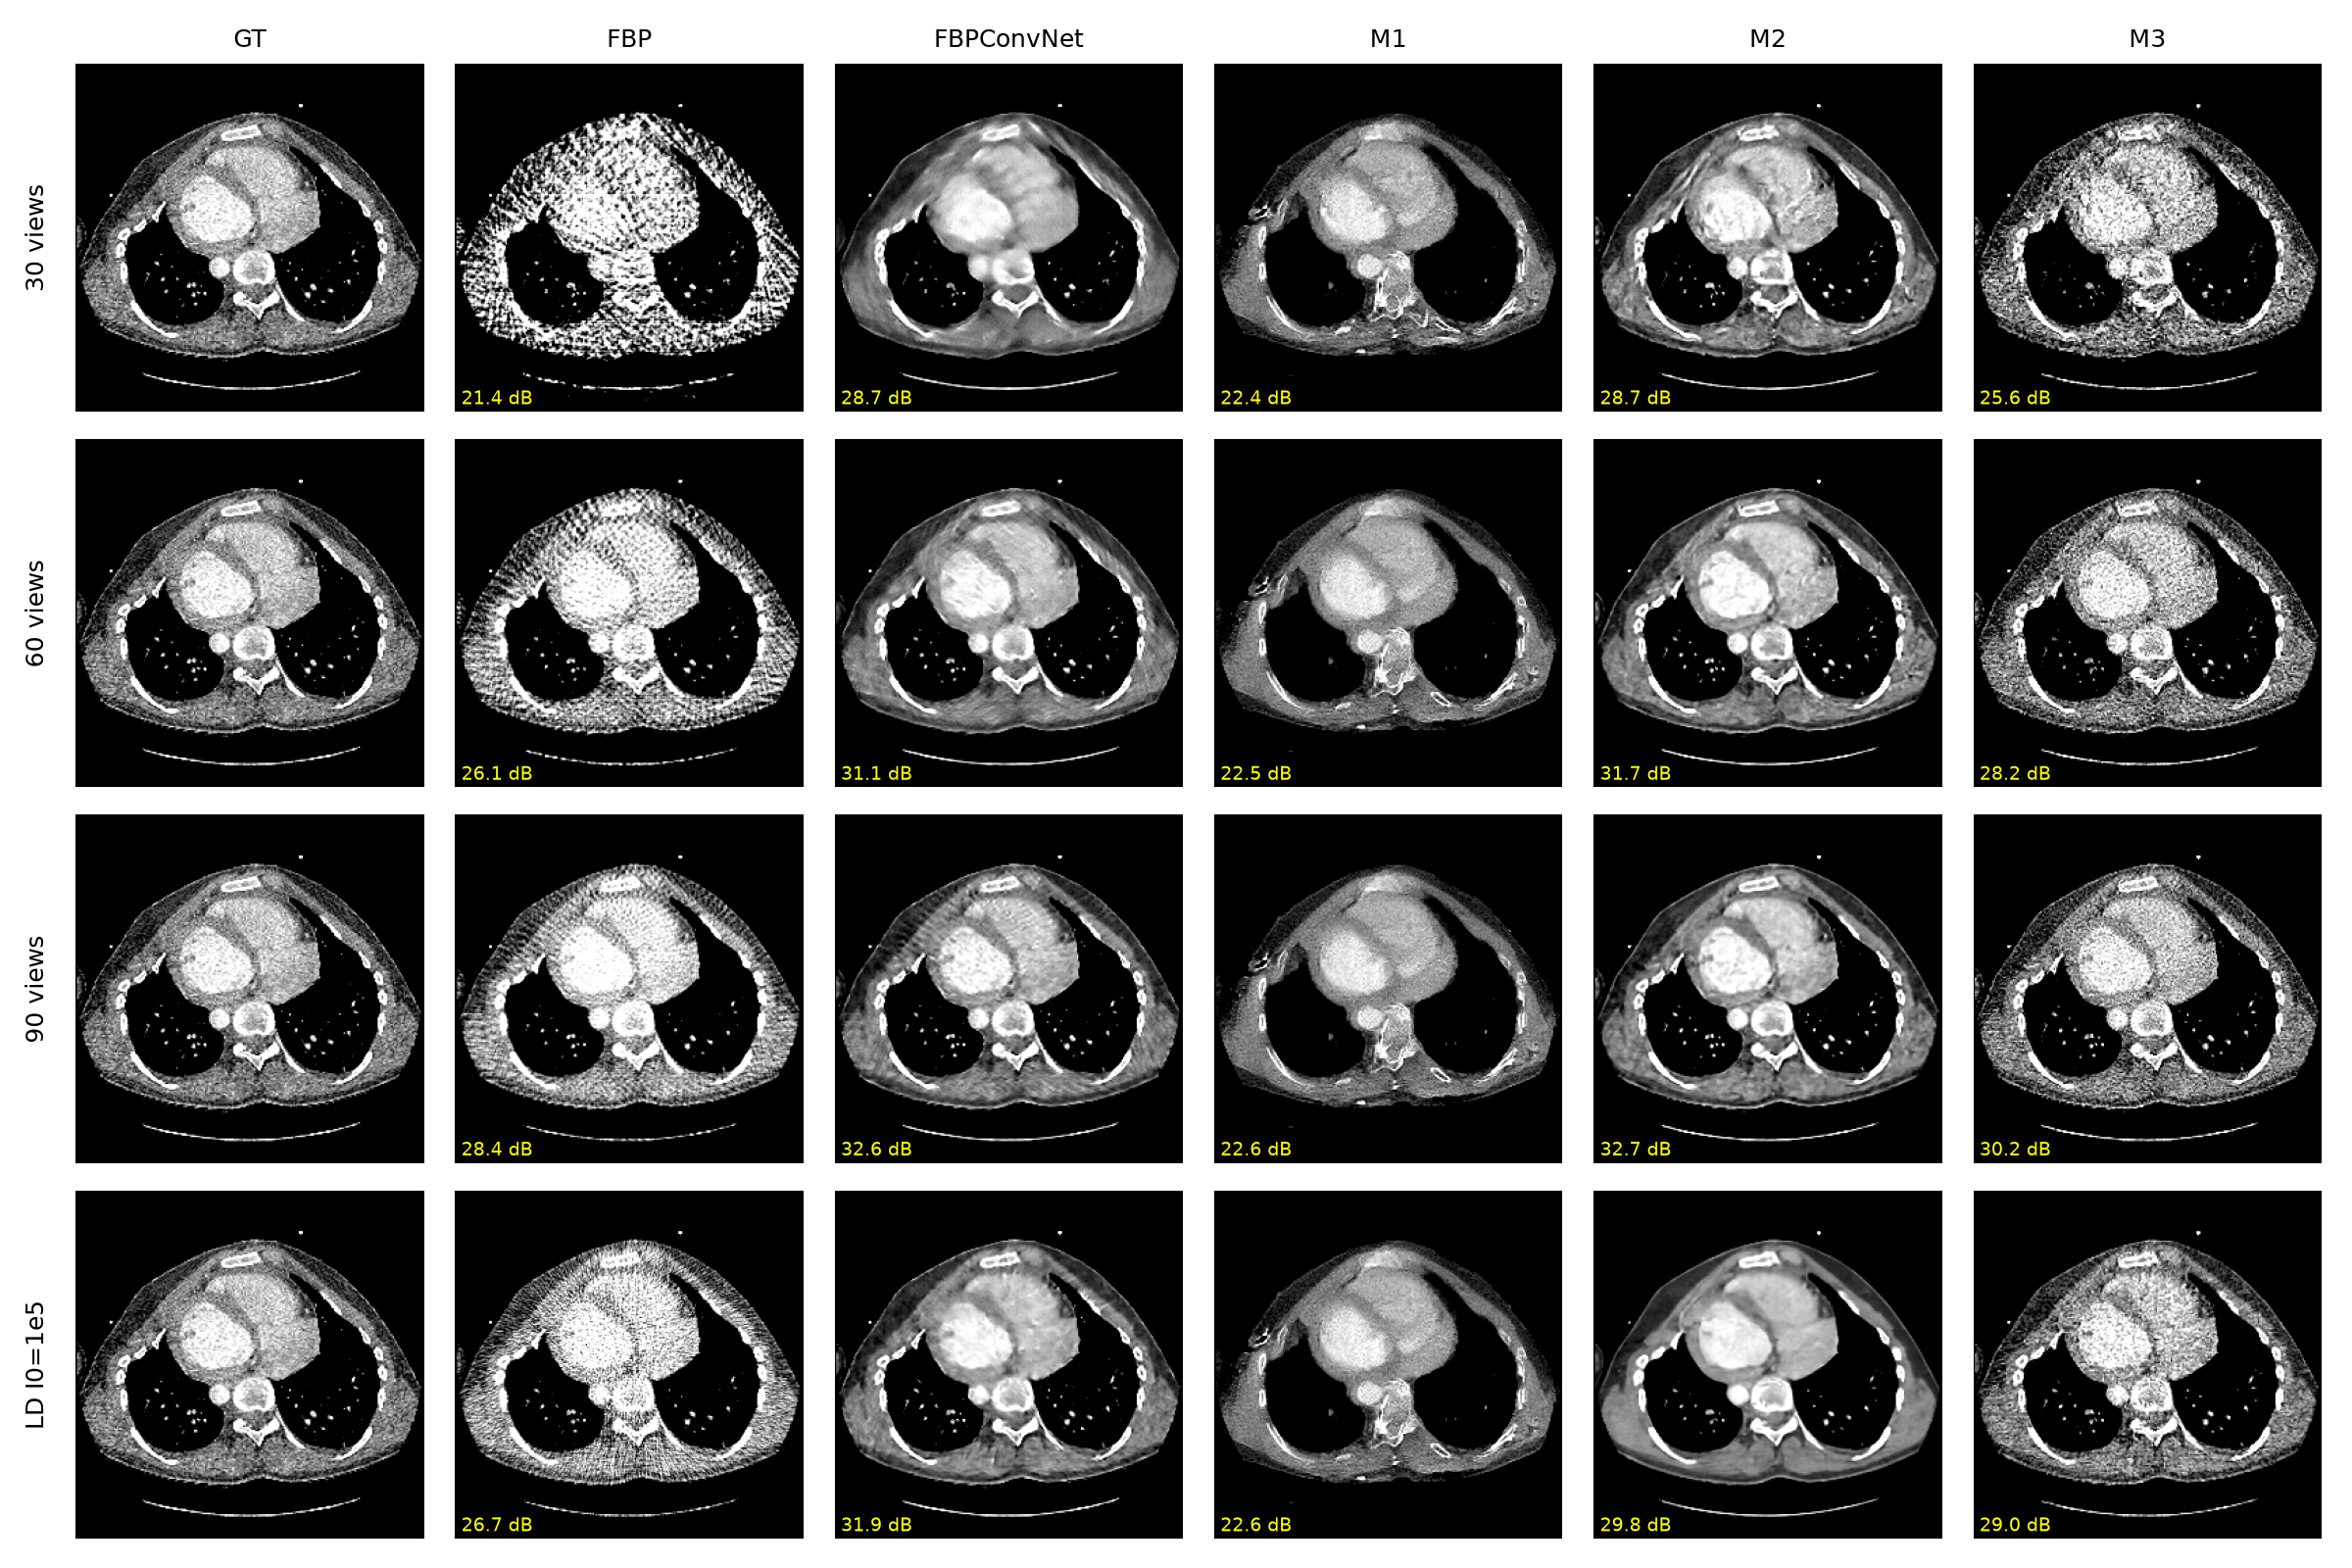
\includegraphics[width=\linewidth]{figures/qualitative.png}
\caption{A thoracic test slice (soft-tissue window W400/L40; outside the reconstruction disk masked). Numbers: PSNR inside
the disk; this noisy clinical scan is below the dataset average (Table~\ref{tab:main}). M1 alters vertebrae and ribs (hallucination); FBPConvNet over-smooths; M2 is sharpest; M3 keeps the noise
texture of the measured scan.}
\label{fig:qual}
\end{figure}

\paragraph{Posterior means reverse the ranking.}
\begin{table}[t]
\centering
\caption{Single sample vs.\ posterior mean over $K$ samples (test200, NFE 50) and mean per-pixel posterior std.
Paired differences with confidence intervals are given in the text.}
\label{tab:mean}
\small
\begin{tabular}{llccc}
\toprule
Setting & Method & single & mean of $K$ & std \\
\midrule
\multirow{3}{*}{60 views, $K{=}8$} & M1 DPS-grad & 24.53 & 26.22 & 0.129 \\
 & M2 $\Pi$GDM & 36.75 & 38.60 & 0.053 \\
  & M3 Prox-DC & 35.95 & \textbf{39.41} & 0.060 \\
\midrule
\multirow{3}{*}{30 views, $K{=}4$} & M1 DPS-grad & 24.50 & 25.86 & 0.123 \\
 & M2 $\Pi$GDM & 31.45 & 33.33 & 0.067 \\
 & M3 Prox-DC & 31.63 & \textbf{34.54} & 0.066 \\
\bottomrule
\end{tabular}
\end{table}
Averaging posterior samples (Table~\ref{tab:mean}) helps all methods, but unevenly: M3 gains 3.5\,dB and overtakes M2,
whose gain is 1.9\,dB (M3$-$M2 on the posterior mean: $+0.82$ $[0.28,1.43]$ at 60 views, $+1.21$ $[0.43,2.04]$ at 30 views).
The posterior std maps (Fig.~\ref{fig:unc}) suggest a reason: M2's uncertainty is small and concentrated on edges and
lung texture, whereas M3's is diffuse and noise-like rather than edge-concentrated, consistent with samples that differ
mainly in components left unconstrained by the data, which average out. Against the supervised network, the posterior
mean of M3 is better by 2.3--3.9\,dB ($[1.65,3.02]$ at 30 and $[2.97,4.95]$ at 60 views) and that of M2 by 1.1--3.1\,dB. Whether a
single sample or a posterior mean is the relevant output therefore decides which rule is preferable.

\begin{figure}[t]
\centering
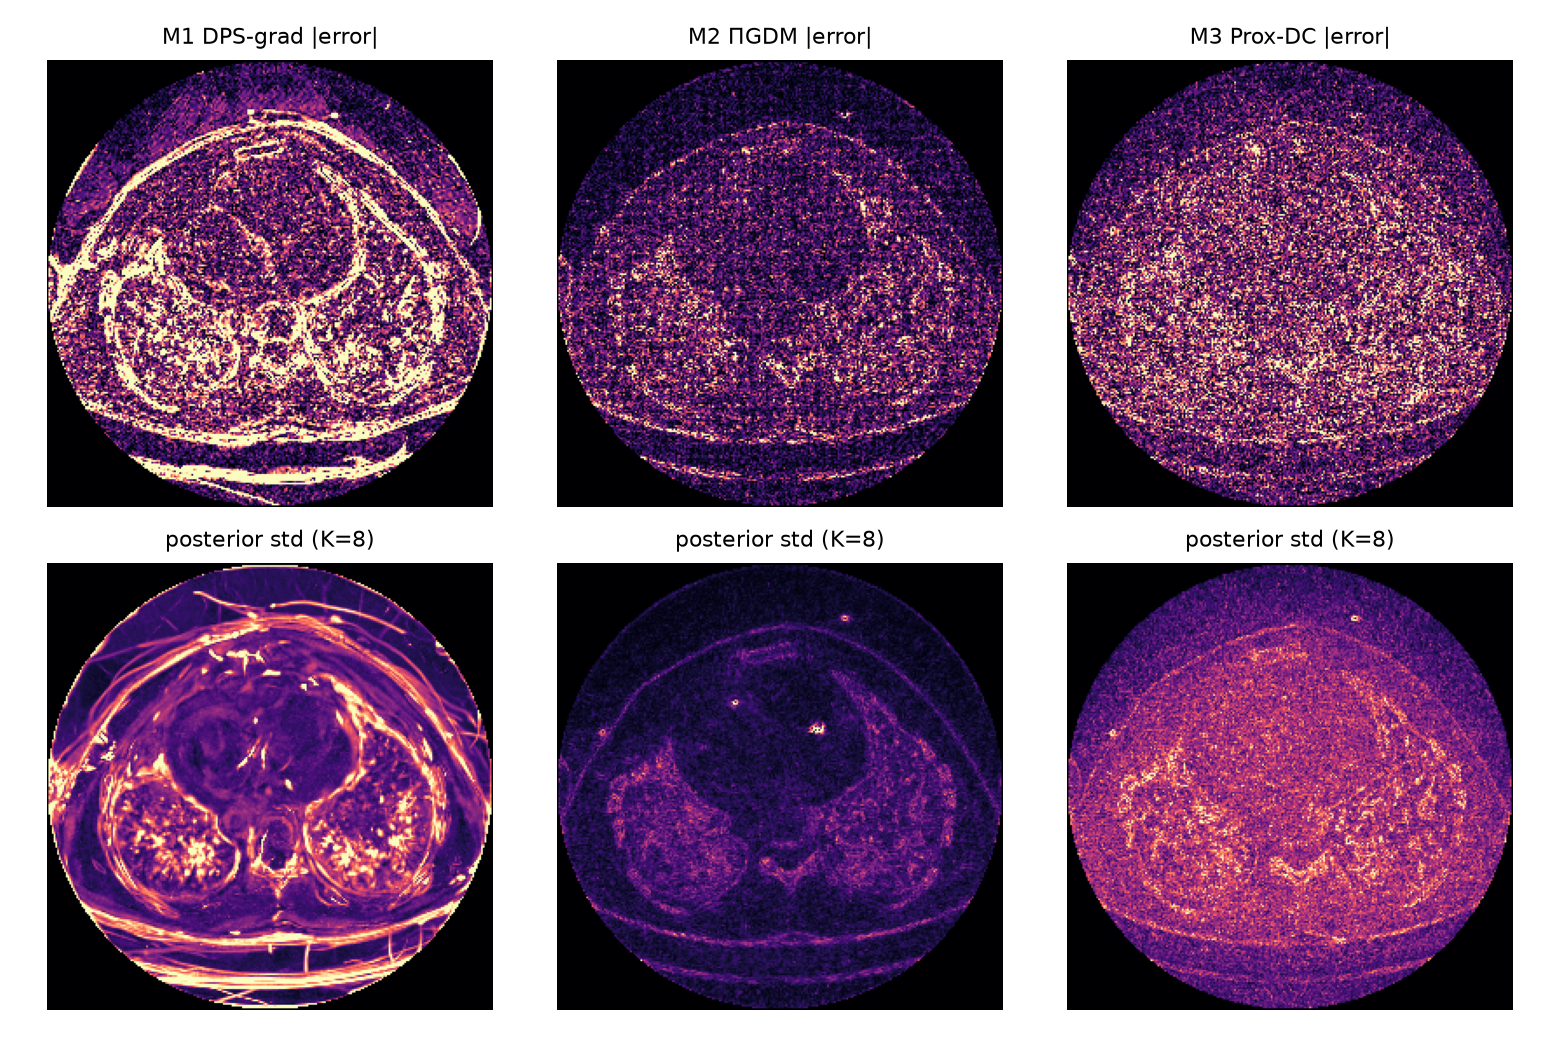
\includegraphics[width=0.85\linewidth]{figures/uncertainty.png}
\caption{Absolute error of one sample (top) and posterior std over 8 samples (bottom), 60 views, same slice as
Fig.~\ref{fig:qual}. M1's error and uncertainty follow anatomy (it generates different structures); M2's uncertainty is
small and concentrated at edges; M3's is noise-like.}
\label{fig:unc}
\end{figure}

\paragraph{Step efficiency.}
Figure~\ref{fig:nfe} varies NFE at 60 views. M3 is already at 36.2\,dB with 20 steps (36\,s for 200 slices) and slightly
\emph{decreases} with more steps (35.7\,dB at 100), consistent with a hard projection being applied more often to noisy
intermediate estimates. M2 benefits from more steps (34.3$\to$37.4\,dB) and is best at 100 steps; M1 improves the most
(19.1$\to$28.1\,dB) but remains below FBP even at 100 steps.

\begin{figure}[t]
\centering
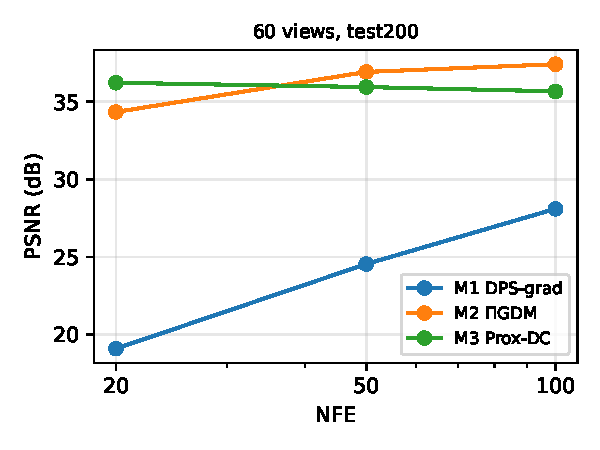
\includegraphics[width=0.45\linewidth]{figures/nfe.pdf}
\caption{PSNR vs.\ NFE at 60 views (test200), with guidance strengths fixed at the values tuned at NFE 50. Thanks to the
$\Delta t$ scaling the integrated guidance is the same at every NFE.}
\label{fig:nfe}
\end{figure}

\paragraph{Why gradient guidance fails on the flow ODE.}
In a preliminary measurement (4 validation slices, 60 views, an intermediate 40k-step checkpoint, NFE 20), the RMS of the
M1 guidance gradient was $\approx1.9$ at $t{=}0$ but $0.03$--$0.07$ for $t\ge 0.2$, a $\sim\!60\times$ drop that we attribute
to the large network Jacobian on pure noise; a measurement with the final checkpoint is left to the next revision. A single $\zeta$ therefore either throws the first step off the data manifold or is too weak later: with
$t_s{=}0$ the best validation PSNR was 13.8\,dB (16 slices, NFE 20), and delaying guidance to $t_s{=}0.2$--$0.4$ is necessary
(Fig.~\ref{fig:tune}). Even when tuned, M1 saturates at $\approx\!24.5$\,dB for 30, 60 and 90 views alike
(Table~\ref{tab:main}). With the gradient of the residual \emph{norm}, the step does not scale with $\|\bm r\|$ and so cannot
shrink as consistency improves; we conjecture that this, together with a constant $\zeta$, rather than the ODE per se, causes
the view-independent plateau. Time-dependent guidance weights~\cite{moroy2026guidanceweights} are the natural remedy and
are left to future work.
Its samples are only coarsely consistent (DC $\approx3.8\%$, comparable to FBP and more than ten times that of M2/M3) and hallucinate anatomy
(Figs.~\ref{fig:qual},~\ref{fig:unc}). M2 and M3, whose corrections vanish with the residual, do not show this behaviour.

\begin{figure}[t]
\centering
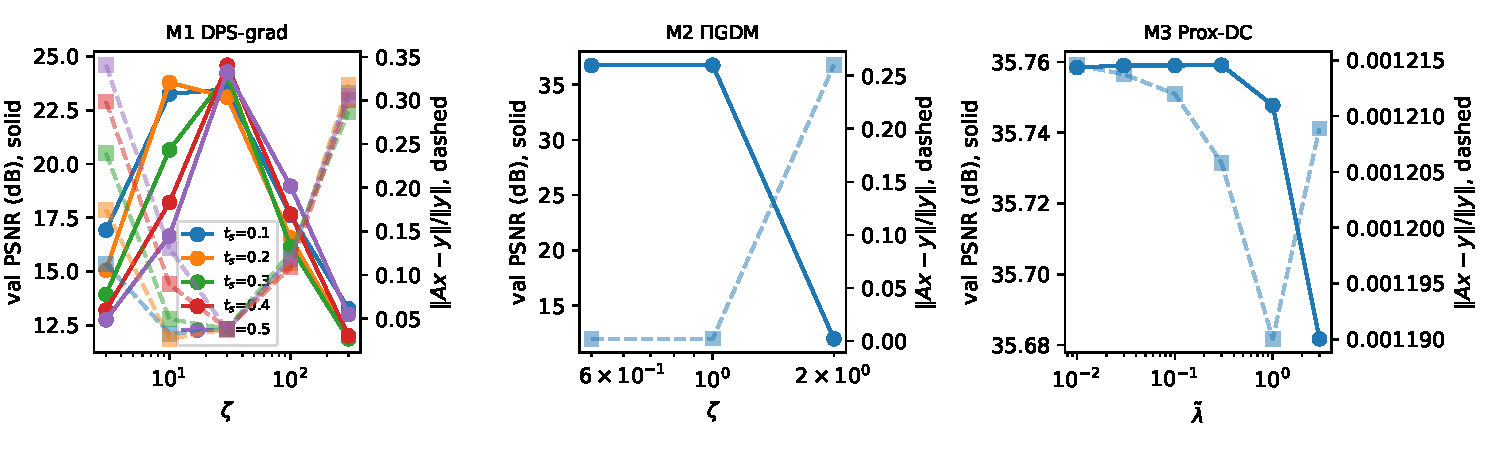
\includegraphics[width=\linewidth]{figures/tuning.pdf}
\caption{Validation PSNR (solid) and data consistency (dashed) vs.\ guidance strength at 60 views. M1: one curve per start
time $t_s$; M2 diverges for $\zeta{=}2$; M3 is insensitive over two decades of $\tilde\lambda$.}
\label{fig:tune}
\end{figure}

\paragraph{Low dose.}
With Poisson noise the picture changes. At $I_0{=}10^5$ the supervised FBPConvNet is best (35.3\,dB), $2.2$\,dB above M2
(CI $[1.86,2.49]$) and 4.7\,dB above M3; M3 needs a strong proximal weight ($\tilde\lambda{=}30$) not to copy noise into the
image. In the photon-starved extreme $I_0{=}10^4$, with strengths transferred from $I_0{=}10^5$ and not re-tuned, the ranking
inverts: FBP 18.0, M3 20.6, M2 22.5 and M1 24.5\,dB---M1 is the most robust, plausibly because it uses the data least.
We deliberately gave M2 and M3 no noise model ($\sigma_y{=}0$, unweighted least squares), which handicaps them under Poisson
noise, whereas FBPConvNet learns the noise statistics implicitly; whether re-tuning or a noise model closes the gap is open.

\paragraph{Sensitivity.}
M3 is the easiest rule to deploy: its validation PSNR varies by less than 0.1\,dB for $\tilde\lambda\in[0.01,1]$ (Fig.~\ref{fig:tune});
in the noiseless setting it effectively acts as a hard projection. M2 has a sharp stability limit (it diverges at
$\zeta{=}2$ for sparse views), and M1 requires a two-dimensional search.

\FloatBarrier
\section{Discussion and limitations}
For flow-matching priors in noiseless sparse-view CT, our results favour rules whose correction vanishes with the residual:
pseudo-inverse guidance for the best single sample at moderate NFE, and proximal consistency for few-step sampling and for
posterior means. Gradient guidance with unit-norm steps, transplanted from diffusion SDEs, is not competitive on the ODE even
when its units and start time are tuned. Under photon noise, both consistency rules need an explicit noise model or
per-dose tuning to match a supervised network.

The study has clear limits. The forward model is a simulated parallel-beam projector applied to reconstructed volumes, so it
is exactly known and matched between training and test; fan/cone-beam geometry, operator mismatch and real projection data
(e.g.\ Mayo LDCT) are not covered. The ground-truth volumes themselves include noisy clinical scans, which caps attainable PSNR
and penalises denoising behaviour. Strengths are tuned once per noise regime and transferred across view counts and doses,
which favours rules whose optimum transfers well; we regard this as part of what is measured. The supervised baseline is
trained with $\approx25\times$ fewer sample passes than the prior, so its numbers are a lower bound. The prior is 2-D and does not
enforce inter-slice consistency~\cite{chung2023diffusionmbir,song2024diffusionblend}; the M1 trajectory analysis uses an
intermediate checkpoint; and posterior-mean results use $K{=}8$ (60 views) and $K{=}4$ (30 views) samples only.

\section*{Code and data availability}
Code, configuration files, per-image metrics and the patient lists of all splits are available at
\url{https://github.com/ZeroDevi1/flow-ct-guidance}. The data are the public TotalSegmentator v2.0.1 collection (CC-BY-4.0).

\section*{Acknowledgments}
The experiment code, the execution of the experiments and the first draft of this manuscript were prepared with the
assistance of an AI coding assistant (Claude, Anthropic). All results and text were checked by the authors, who take
full responsibility for the content.

\bibliographystyle{unsrtnat}
\bibliography{references}
\end{document}
